\documentclass[12pt]{article}
\usepackage{amsmath} % AMS Math Package
\usepackage{bm}
\usepackage{amsthm} % Theorem Formatting
\usepackage{amssymb}    % Math symbols such as \mathbb
\usepackage{graphicx} % Allows for eps images
\usepackage[dvips,letterpaper,margin=1in,bottom=0.7in]{geometry}
\usepackage{tensor}
\usepackage{amsmath}
\usepackage{siunitx}
\usepackage{physics}
\usepackage{setspace}

\newtheorem{p}{Problem}
\usepackage{cancel}
\newtheorem*{lem}{Lemma}
\theoremstyle{definition}
\newtheorem*{dfn}{Definition}
 \newenvironment{s}{%\small%
        \begin{trivlist} \item \textbf{Solution}. }{%
            \hspace*{\fill} $\blacksquare$\end{trivlist}}%


\begin{document}

{\noindent\Huge\bf  \\[0.5\baselineskip] {\fontfamily{cmr}\selectfont  Exam 2}         }\\[2\baselineskip] % Title
{ {\bf \fontfamily{cmr}\selectfont Quantum Mechanics}\\ {\textit{\fontfamily{cmr}\selectfont     \today}}}~~~~~~~~~~~~~~~~~~~~~~~~~~~~~~~~~~~~~~~~~~~~~~~~~~~~~~~~~~~~~~~~~~~~~~~~~~~~~    {\large \textsc{C Seitz}
\\[1.4\baselineskip] 

\begin{p}
\end{p}

\begin{s}

Some of the states have the same energy, so we will need to use degenerate perturbation theory. Specifically, the subspaces spanned by $\mathcal{A} = \{\ket{0^{(0)}},\ket{1^{(0)}}\}$ and $\mathcal{B} = \{\ket{2^{(0)}},\ket{4^{(0)}}\}$ have a degeneracy while the lone ket $\ket{3^{(0)}}$ is nondegenerate. We assume that a perturbed ket $\alpha \in \mathcal{A}$ can be written as a linear combination of the unperturbed kets:

\begin{align*}
\ket{\alpha} = \sum_{n\in \mathcal{A}}\bra{n}\ket{\alpha}\ket{n}
\end{align*}

The first order correction is given by

\begin{align*}
V\ket{\alpha} = \sum_{n\in \mathcal{A}}\bra{n}\ket{\alpha}(H-H_{0})\ket{n} = \Delta_{\alpha}^{(1)}\ket{\alpha}
\end{align*}

We therefore need to find the eigenvectors and eigenvalues of the matrix

\begin{align*}
|V_{\mathcal{A}} - \Delta_{\alpha} I| = \mathrm{det}\begin{pmatrix}
2\cos\theta - \Delta_{\alpha}& 2\sin\theta e^{-i\phi}\\
2\sin\theta e^{i\phi} & -2\cos\theta- \Delta_{\alpha}
\end{pmatrix} = 0
\end{align*}

which is easy to solve, and we get the first order shifts $\Delta_{\alpha}^{(1)} = \pm 2$. It is the same process for the $\mathcal{B}$ subspace

\begin{align*}
|V_{\mathcal{B}} - \Delta_{\beta} I| = \mathrm{det}\begin{pmatrix}
4\cos\theta - \Delta_{\beta}& 4\sin\theta e^{-i\phi}\\
4\sin\theta e^{i\phi} & -4\cos\theta- \Delta_{\beta}
\end{pmatrix} = 0
\end{align*}

It is pretty much the same matrix, so $\Delta_{\beta}^{(1)} = \pm 4$. For the first order correction to the nondegnerate ket $\ket{3^{(0)}}$, we use nondegenerate perturbation theory to first order

\begin{align*}
\Delta_{3}^{(1)} &= \lambda V_{33} + \lambda^{2}\sum_{j\neq 3}\frac{|V_{j3}|^{2}}{E_{3}^{(0)}-E_{j}^{(0)}}\\
&= \lambda + \lambda^{2}\left(-\frac{3}{\epsilon}-\frac{3}{\epsilon}\right)\\
&= \lambda - \frac{6\lambda^{2}}{\epsilon} \approx \lambda
\end{align*}

To get the corrections to the ground state eigenvector, we can again use nondegenerate perturbation theory 

\begin{align*}
\ket{3^{(1)}} &= \lambda\ket{3^{(0)}} + \lambda^{2}\sum_{j\neq 3}\ket{j^{(0)}}\frac{V_{j3}}{E_{3}^{(0)}-E_{j}^{(0)}}\\
&= \lambda\ket{3^{(0)}} + \frac{\lambda^{2}}{\epsilon}\left(\ket{2^{(0)}}+\ket{4^{(0)}}\right)
\end{align*}

In the limit $\lambda \rightarrow 0$, the eigenvectors are the ``good" linear combinations. To find them we need to find the eigenvectors of the submatrices $V_{\mathcal{A}}$ and $V_{\mathcal{B}}$. 

\end{s}

\begin{p}

\begin{align*}
\ket{\alpha_{\pm}} &= \frac{1}{\sqrt{2}}\left(\ket{0}\pm \ket{1}\right)\\
\ket{\beta_{\pm}} &= \frac{1}{\sqrt{2}}\left(\ket{0}\pm i\ket{1}\right)
\end{align*}

\end{p}

\begin{s}
We are after the ensemble expectation values $[x^{n}]$ and $[p^{n}]$. In general, 

\begin{align*}
[A] = \sum_{n}w_{n}\bra{\alpha_{n}}A\ket{\alpha_{n}}
\end{align*}

If the entire ensemble is prepared in the state $\ket{\alpha_{+}}$, then $[x^{n}]$ and $[p^{n}]$ are

\begin{align*}
[x^{n}] &= \bra{\alpha_{+}}x^{n}\ket{\alpha_{+}}\\
&= \frac{1}{2}\left(\bra{0}+ \bra{1}\right)x^{n}\left(\ket{0}+ \ket{1}\right)\\
&= \sqrt{\frac{\hbar}{8m\omega}}\left(\bra{0}+ \bra{1}\right)\left(a+a^{\dagger}\right)^{n}\left(\ket{0}+ \ket{1}\right)\\
\end{align*}


\begin{align*}
[A] = \mathrm{Tr}(\rho A)
\end{align*}

where $\rho$ is the density matrix

\begin{align*}
\rho = \sum_{n}w_{n}\ket{\alpha_{n}}\bra{\alpha_{n}}
\end{align*}

If the entire ensemble is prepared in the state $\ket{\alpha_{+}}$, 

\begin{align*}
\rho &= \ket{\alpha_{+}}\bra{\alpha_{+}}\\
&= \frac{1}{2}\left(\ket{0}+ \ket{1}\right)\left(\bra{0}+ \bra{1}\right)\\
&= \frac{1}{2}\left(\ket{0}\bra{0} + \ket{0}\bra{1} + \ket{1}\bra{0} + \ket{1}\bra{1}\right)
\end{align*}


\end{s}

\begin{p}
\end{p}

\begin{s}
In this two particle system, we have $j_{1} = 1$ and $j_{2} = 2$. We are told the $z$ component of the individual angular momenta $m_{1} = -1$ and $m_{2} = 2$. So we use the state kets $\ket{j_{1}, j_{2}; m_{1},m_{2}}$ where $m_1$ and $m_2$ follow the usual rules. So the state is $\ket{1,2;-1,2}$.

\begin{align*}
\langle J^{2} \rangle &= \bra{1,2;-1,2}J^{2}\ket{1,2;-1,2}\\
&= \bra{1,2;-1,2}\left(J_{1}^{2}+J_{2}^{2} + 2J_{1z}J_{2z}\right)\ket{1,2;-1,2}\\
&= j_{1}(j_{1}+1)\hbar^{2} + j_{2}(j_{2}+1)\hbar^{2} - 4\hbar^{2}\\
&= 2\hbar^{2} + 6\hbar^{2} - 4\hbar^{2}\\
&= 4\hbar^{2}
\end{align*}

We cannot directly compute the expectation values of $J_x, J_y, J_z$ in this basis, because $\ket{j_1, j_2, m_1, m_2}$ are not eigenkets of $J_x, J_y, J_z$. But can change basis:

\begin{align*}
\ket{j_1, j_2, m_1, m_2} = \sum_{m_1,m_2} \ket{j_1,j_2; jm}\bra{j_1,j_2; jm}\ket{j_{1}, j_{2}; m_{1},m_{2}}
\end{align*}

We need to determine $\bra{j_1,j_2; jm}\ket{j_{1}, j_{2}; m_{1},m_{2}}$ which are the Clebsch-Gordon coefficients.

\begin{figure}
\centering
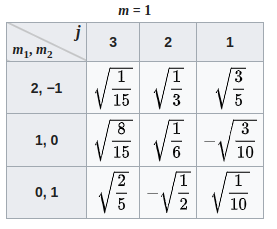
\includegraphics[scale=0.75]{cb-table.png}
\caption{Clebsch-Gordon coefficients for $j_{1} = 1$, $j_{2} = 2$, $m=1$}
\end{figure}

Noting that $m = m_1 + m_2 = 1$, we find

\begin{align*}
\ket{1,2;-1,2} = \sqrt{\frac{3}{5}}\ket{1,2;1 1} + \sqrt{\frac{1}{3}}\ket{1,2;2 1} + \sqrt{\frac{1}{15}}\ket{1,2;3 1}
\end{align*}

The expectation value $\langle J_z \rangle$ is then

\begin{align*}
\langle J_z \rangle &= \bra{1,2;-1,2} J_z \ket{1,2;-1,2} \\
&= \left(\sqrt{\frac{3}{5}}\bra{1,2;1 1} + \sqrt{\frac{1}{3}}\bra{1,2;2 1} + \sqrt{\frac{1}{15}}\bra{1,2;3 1}\right)J_{z}\\
&\left(\sqrt{\frac{3}{5}}\ket{1,2;1 1} + \sqrt{\frac{1}{3}}\ket{1,2;2 1} + \sqrt{\frac{1}{15}}\ket{1,2;3 1}\right)\\
&= \hbar\left(\frac{3}{5}+\frac{1}{3}+\frac{1}{15}\right) = \hbar
\end{align*}

as we should expect. For $J_x, J_y$, 

\begin{align*}
\langle J_x \rangle &= \bra{1,2;-1,2} J_x \ket{1,2;-1,2} \\
&= \left(\sqrt{\frac{3}{5}}\bra{1,2;1 1} + \sqrt{\frac{1}{3}}\bra{1,2;2 1} + \sqrt{\frac{1}{15}}\bra{1,2;3 1}\right)\\
&\frac{1}{2}\left(J_+ + J_-\right)\left(\sqrt{\frac{3}{5}}\ket{1,2;1 1} + \sqrt{\frac{1}{3}}\ket{1,2;2 1} + \sqrt{\frac{1}{15}}\ket{1,2;3 1}\right)\\
&= 0
\end{align*}

and $\langle J_{y} \rangle = 0$ since neither $J_+$ nor $J_-$ connects two $\ket{j_1,j_2;jm}$ states.

Now, if we measure the total angular momentum and obtain the largest possible value, then we are in the state $\ket{1,2;31}$ in the $\ket{j_1,j_2;jm}$ basis. However, to compute $J_{1z}$ and $J_{2z}$ we need to transform this back to the $\ket{j_1, j_2, m_1, m_2}$ basis. Looking up the coefficients, we get

\begin{align*}
\ket{1,2;31} = \left(\sqrt{\frac{1}{15}}\ket{1,2;-12} + \sqrt{\frac{2}{5}}\ket{1,2;10} + \sqrt{\frac{8}{15}}\ket{1,2;01}\right)
\end{align*}

\begin{align*}
\langle J_{1z} \rangle &= \bra{1,2;31} J_{1z}  \ket{1,2;31} \\
&= \left(\sqrt{\frac{1}{15}}\bra{1,2;-12} + \sqrt{\frac{2}{5}}\bra{1,2;10} + \sqrt{\frac{8}{15}}\bra{1,2;01}\right)\\
&J_{1z}\left(\sqrt{\frac{1}{15}}\ket{1,2;-12} + \sqrt{\frac{2}{5}}\ket{1,2;10} + \sqrt{\frac{8}{15}}\ket{1,2;01}\right)\\
&= -\hbar\frac{1}{15} + \hbar\frac{2}{5} =  \frac{\hbar}{3}
\end{align*}

\begin{align*}
\langle J_{2z} \rangle &= \bra{1,2;31} J_{2z}  \ket{1,2;31} \\
&= \left(\sqrt{\frac{1}{15}}\bra{1,2;-12} + \sqrt{\frac{2}{5}}\bra{1,2;10} + \sqrt{\frac{8}{15}}\bra{1,2;01}\right)\\
&J_{2z}\left(\sqrt{\frac{1}{15}}\ket{1,2;-12} + \sqrt{\frac{2}{5}}\ket{1,2;10} + \sqrt{\frac{8}{15}}\ket{1,2;01}\right)\\
&= 2\hbar\frac{1}{15} + \hbar\frac{8}{15} = \frac{2\hbar}{3}
\end{align*}

The probability that $J_{1z}$ and $J_{2z}$ never change from their original values is given by 

\begin{align*}
|\bra{1,2;-12}\ket{1,2;31}|^{2} = 1/15
\end{align*}

\begin{figure}
\centering
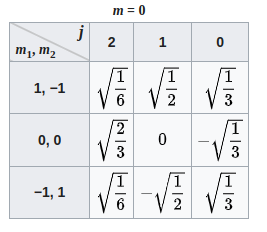
\includegraphics[scale=0.75]{cb-table-2.png}
\caption{Clebsch-Gordon coefficients for $j_{1} = 1$, $j_{2} = 1$ and $m=0$}
\end{figure}

If we instead measure the smallest possible value, we are in state $\ket{1,2;11}$. The third particle being added has $j_{3} = 1$ and $m_{3} = -1$. We can consider the first two particles as a single composite particle in state $\ket{jm} = \ket{11}$. We now have two particles with $j = 1$. Taking $m_{1} = 1$ and $m_{2} = -1$ and reading off the table above, the probabilities are

$$
\mathbf{Pr}(j)=
\begin{cases}
\frac{1}{3}, j = 0 \\
\frac{1}{2}, j = 1 \\
\frac{1}{6}, j = 2 \\
\end{cases}
$$

Finally, the expectation value of $J^{2}$ for this three particle system is 

\begin{align*}
\langle J^{2} \rangle &= \bra{1,1;1,-1}J^{2}\ket{1,1;1,-1}\\
&= \bra{1,1;1,-1}\left(J_{1}^{2}+J_{2}^{2} + 2J_{1z}J_{2z}\right)\ket{1,1;1,-1}\\
&= j_{1}(j_{1}+1)\hbar^{2} + j_{2}(j_{2}+1)\hbar^{2} - 2\hbar^{2}\\
&= 2\hbar^{2}
\end{align*}

\end{s}

\end{document}